% Copyright (c) 2022 Tobias Briones. All rights reserved.
%
% SPDX-License-Identifier: CC-BY-SA-4.0
%
% This file is part of Course Project at UNAH-IS911: Microprocessors.
%
% This source code is licensed under the Creative Commons Attribution Share
% Alike 4.0 International License found in the LICENSE file in the root
% directory of this source tree or at https://spdx.org/licenses/CC-BY-SA-4.0.

\documentclass[conference]{IEEEtran}
\usepackage[letterpaper, portrait, margin=2cm]{geometry}
\usepackage[style=ieee]{biblatex}
\usepackage[utf8]{inputenc}
\usepackage[spanish]{babel}
\usepackage{geometry}
\usepackage[]{graphics}
\usepackage[demo]{graphicx}
\usepackage{csquotes}
\usepackage{float}
\usepackage{hyperref}
\usepackage[table,xcdraw]{xcolor}
\usepackage{lipsum}

\addbibresource{bibliography.bib}

\title{Microcontrolado PIC}
\author{
    
\includegraphics[width = 40mm]{images/logo-unah.png}\\[8ex]
    \IEEEauthorblockN{Tobias Briones}
    \IEEEauthorblockN{tobias.briones@unah.hn}
    \IEEEauthorblockA{\textit{Universidad Nacional Autónoma de Honduras} \\
    \textit{Ingeniería de Sistemas} \\
    \textit{I PAC 2022} \\
    \textit{IS911-MICROPROCESADORES}} \\\vspace*{20pt} \normalsize  \\
    \today
}

\hypersetup{
    colorlinks=true,
    linkcolor=black,
    filecolor=magenta,
    urlcolor=cyan,
    citecolor=black
}

\newcommand\blfootnote[1]{%
    \begingroup
    \renewcommand\thefootnote{}\footnote{#1}%
    \addtocounter{footnote}{-1}%
    \endgroup
}

\begin{document}

    \maketitle

    \begin{abstract}
    \end{abstract}

    \tableofcontents

    \blfootnote{
        Copyright (c) 2022 Tobias Briones. All rights reserved. \\
        This work is licensed under the Creative Commons Attribution Share Alike 4.0 International License (\href{https://spdx.org/licenses/CC-BY-SA-4.0}{CC-BY-SA-4.0}). \\
        Third party contents available under their respective copyright and license.\\
        For more details go to the \href{https://github.com/tobiasbriones/cp-unah-is911-microprocessors}{GitHub Repository}.}

    \section{Introducción}

    Los PIC son una familia de microcontroladores desarrollados por Microchip Technologies \cite{microchip-technology-inc-2013} los cuales son muy conocidos y utilizados tanto a nivel educativo como industrial. Cualquiera que está interesado en el aprendizaje o implementación de circuitos electrónicos, IoT o sistemas embebidos definitivamente debió de haber conocido o utilizado estos microcontroladores ya que son tan populares como las tarjetas Arduino. Así mismo, tienen una gran historia por detrás que data desde el año $1976$ y según wikipedia tenemos que \cite{wikipedia-pic-2022}:

    \bigbreak

    \begin{quote}
        \textbf{PIC} (generalmente pronunciado como "pick") es una familia de microcontroladores fabricados por Microchip Technology, derivados del PIC1650 desarrollado originalmente por la División de Microchip de General Instrument (GI). El nombre PIC inicialmente se refería a Controlador de Interfaz Periférico, y actualmente se expande como Computadora Inteligente Programable. Las primeras partes de la familia estuvieron disponibles en 1976; en 2013, la empresa había enviado más de doce mil millones de piezas individuales, utilizadas en una amplia variedad de sistemas integrados.
        \\
        \small Fuente: Wikipedia $\mid$ PIC microcontrollers (traducido de inglés a español) \cite{wikipedia-pic-2022}
    \end{quote}

    Los PICs han evolucionado en el tiempo. Por ejemplo, algunos modelos iniciales usaban la ROM directamente (o como se dice hard-coded o hard-written) para almacenar el código pero luego los modelos actuales empezaron a utilizar EPROM y EEPROM, ahora memoria flash y por último el PIC permite que se reprograme solo \cite{wikipedia-pic-2022}. Esto implica una gran ventaja para el programador humano.

    \bigbreak

    El IDE que utilizan los PICs es un software propietario del proveedor Microchip Technologies el cual permite lenguaje ensamblador y C/C++ \cite{microchip-technology-inc-2013} \cite{wikipedia-pic-2022}. Aunque otros lenguajes de bajo nivel como Rust \footnote{A veces causa polémica decir que un lenguaje es de bajo nivel. Yo lo defino como tomar el subconjunto (unsafe) del lenguaje que lo hace de bajo nivel (o framework de ensamblador) o simplemente referirse como \say{lenguaje de más bajo nivel}.} también se pueden emplear para programar dispositivos sin sistema operativo (\say{el metal}) pero hay que tener en cuenta que puede haber falta de soporte para las arquitecturas de CPU y compiladores u otras herramientas.

    \begin{figure}[H]
        \centering
        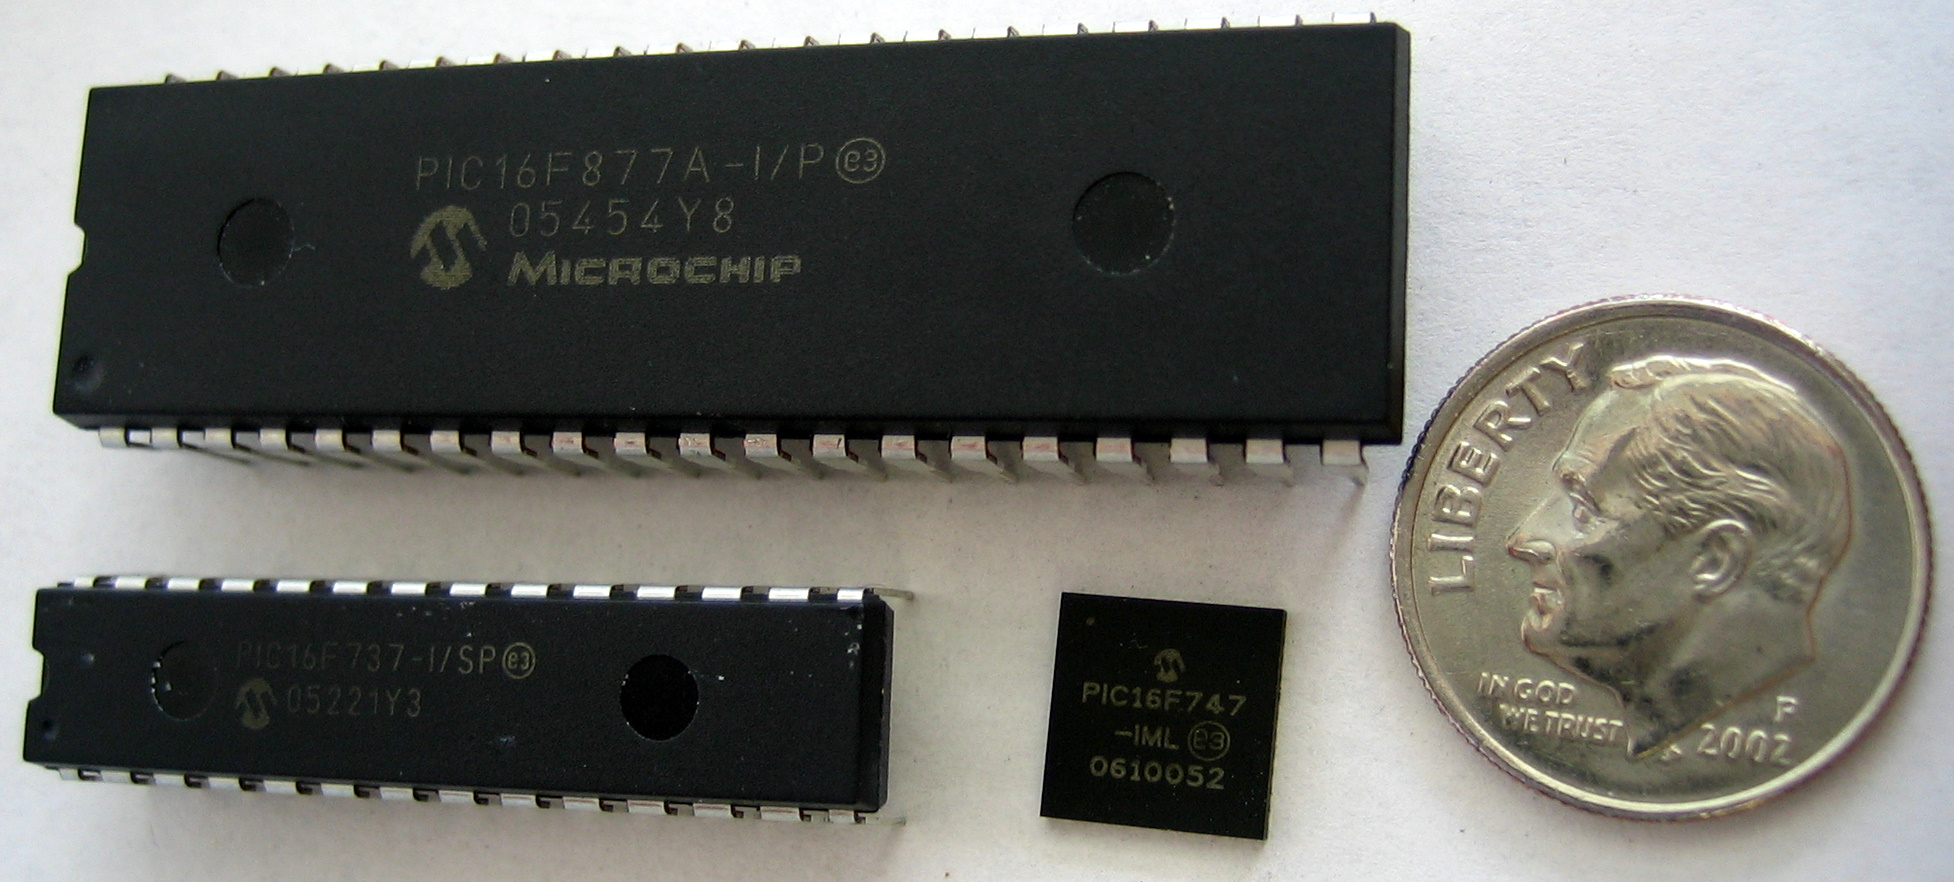
\includegraphics[width=0.3\paperwidth]{images/pic-microcontrollers.jpg}
        \caption{Microcontroladores PIC} \footnotesize
        Fuente: Wikipedia $\mid$ Por MikeMurphy, dominio público, https://commons.wikimedia.org/w/index.php?curid=1225813 \cite{wikipedia-pic-2022}
    \end{figure}

    \printbibliography

\end{document}
